\documentclass[conference]{IEEEtran}
\IEEEoverridecommandlockouts
\usepackage{cite}
\usepackage{amsmath,amssymb}
\usepackage{booktabs}
\usepackage{graphicx}
\usepackage{xcolor}
\usepackage{url}
\usepackage[hidelinks]{hyperref}
\usepackage{balance}
\usepackage{pgfplots}
\pgfplotsset{compat=1.16}

\newcommand{\gate}[1]{\texttt{#1}}
\newcommand{\code}[1]{\texttt{\small #1}}

\begin{document}

\title{Probabilistic Reference Monitors: An Empirical Study of Calibrated Decision Models in the Authorization Path of Coding Agents}

% AGENT @ ICSE 2027 is single-anonymous: author names and affiliations must be shown.
\author{\IEEEauthorblockN{\textcolor{red}{TODO: author names}}
\IEEEauthorblockA{\textcolor{red}{TODO: affiliation, email}}}

\maketitle

\begin{abstract}
Coding agents increasingly guard their own dangerous actions with a remote,
probabilistic decision model: a hosted classifier is asked ``is this safe?'' and the
answer, thresholded, decides whether a tool call runs. This inverts the security
literature's requirement that per-call authorization be deterministic, fail-closed, and
outside the untrusted model. We conduct the first empirical study of what practitioners
actually built. We assemble a corpus of 31 public gates at pinned commits and read every
threshold, error path, and action set; we build a 346-item tool-call risk benchmark and
measure the vendor model live; we inject faults into each gate's own code to observe its
failure behaviour; and we run three real gates end to end against the live model. Four
findings stand out. (i) A gate's real-world protection is set not by the model but by the
gate-mode $\times$ host-permission-mode combination: the same gate auto-allows 3 versus 88
of 131 clearly-destructive calls depending on one configuration flag, because ``ask''
verdicts are silently downgraded to ``allow'' when nothing prompts a human. (ii) The
vendor's illustrative $0.9$ threshold, shipped verbatim by 8 gates, auto-allowed \emph{zero}
of 346 items: the model separates safe from destructive perfectly, but its ``safe'' scores
never reached $0.9$. Five weeks later the next model version auto-allows 27\% of safe items at
the same constant, with no change to any gate: a copied threshold's meaning drifts with the
model behind it. (iii) An availability fault is an authorization bypass: padding a
destructive command to exceed the model's token limit returns HTTP~400 in ${\sim}0.7$\,s,
and fail-open gates then execute it---confirmed live end to end. (iv) These pathologies are
not vendor-specific; they recur in non-Jev LLM-judge gates and in the host's own
documented fail-open-on-timeout behaviour, while deterministic gates have no such
availability axis. We give a small, distribution-free recipe that certifies an auto-allow
threshold from ${\sim}40$ labelled calls, recovering 42\% auto-allow at a certified
$\leq 3.1\%$ false-allow rate where the vendor's number certified none. All predictions
were pre-registered; raw call logs, code, and replay scripts are released.
\end{abstract}

\begin{IEEEkeywords}
agentic AI, agentic engineering, authorization, LLM guardrails, calibration,
empirical study, mining software repositories
\end{IEEEkeywords}

\section{Introduction}
A coding agent that can run shell commands, edit files, and call the network needs a way to
decide, per action, whether to proceed. The security literature is unambiguous about how:
per-call authorization must be deterministic, fail-closed, default-deny, and placed outside
the untrusted model that proposes the action~\cite{saltzer1975,scopegate2026,agentspec2026}.
A reference monitor is trustworthy precisely because it does not itself guess.

A new class of tools does the opposite. Following the launch of typed ``decision models''
such as Jev~\cite{jevdocs}, practitioners wire a \emph{remote, probabilistic} model into the
permission path: the model is asked a typed question (``is it safe to run this without
asking?''), returns a probability, and a threshold turns that probability into
allow/ask/deny. The model is documented as jagged on adversarial input, is reached over the
network, and is placed squarely inside the trust boundary it is meant to defend. Dozens of
such gates are public. Nobody has studied what they actually built, how they behave when the
model is slow or wrong, or whether their thresholds mean anything.

We provide that study. We treat a probabilistic model placed in the permission path as the
unit of analysis, with Jev as the first ecosystem where many such gates can be observed at
once, and we ask four questions an operator should be able to answer before trusting one:
(Q1) what did these gates ship---thresholds, error paths, action sets? (Q2) how does the
underlying model behave on a controlled authorization workload? (Q3) what does each gate do
when the model times out, rate-limits, errors, or returns garbage? (Q4) end to end, how many
dangerous actions does a real gate let through, and why?

Our contributions are:
\begin{itemize}
\item A \textbf{corpus} of 31 public gates at pinned commits with hand-verified thresholds,
provenance, error paths, and action sets (Sec.~\ref{sec:corpus}).
\item A \textbf{live behavioural benchmark} (346 items + 80 held-out adversarial) of the
vendor model under four gate configurations, showing the shipped $0.9$ threshold has a dead
auto-allow path (Sec.~\ref{sec:bench}).
\item A \textbf{fault-injection harness} that runs each gate's own code against injected
model faults, correcting a static ``fail-open'' label into a finer taxonomy and confirming
an availability-to-authorization bypass live (Sec.~\ref{sec:fault}).
\item A \textbf{live end-to-end cross-evaluation} of three real gates, showing that
protection is governed by the gate-mode $\times$ host-mode combination, not the model
(Sec.~\ref{sec:live}).
\item A \textbf{constructive fix}: a distribution-free recipe that certifies an auto-allow
threshold from a small labelled set (Sec.~\ref{sec:fix}), and a \textbf{non-Jev comparison}
showing the pathologies generalize (Sec.~\ref{sec:general}).
\end{itemize}
All predictions were pre-registered before data collection. Code, raw call logs, and replay
scripts accompany the paper.

\section{Background and Related Work}
\textbf{Deterministic enforcement.} A line of work re-establishes that agent authorization
must be deterministic and fail-closed: capability/authorization separation~\cite{scopegate2026},
runtime enforcement DSLs~\cite{agentspec2026}, and the classical reference-monitor
requirements of complete mediation and fail-safe defaults~\cite{saltzer1975}. Our gates
violate these by construction; we measure the consequences rather than re-argue the
principle.

\textbf{Models in the decision path.} LLM-as-judge gates are studied as benchmarks
(TraceSafe~\cite{tracesafe2026}), pre-execution gates (ScopeJudge~\cite{scopejudge2026},
CARE~\cite{care2026}), and human-oversight calibration
(Oversight Has a Capacity~\cite{oversight2026}). These evaluate purpose-built judges on
author-constructed inputs. Concurrent work evaluates System One models themselves for
security decisions, finding that strict miss budgets leave little to
automate~\cite{liu2026systemone}, that the option labels of a typed question are an attack
channel~\cite{azizi2026option}, and that LLM gates misjudge benign authorized
requests~\cite{authgatebench2026}; frameworks now pair deterministic state checks with a
decision model~\cite{jevact2026}. All of these study the model or a purpose-built gate. We
instead study \emph{deployed} gates and their failure and availability behaviour, which this
line does not touch. (Azizi et al.\ use ``fail-open'' for a wrong allow; we use it for
behaviour when the model call fails.)

\textbf{Calibration and selective risk.} Guard models are known to be
miscalibrated~\cite{guardcal2025}; selective classification and the cost-optimal reject
threshold are classical~\cite{chow1970,elyaniv2010,guo2017}. Our threshold recipe is
Chow's rule instantiated for authorization with a finite-sample
guarantee~\cite{clopper1934}; we claim the audit and the recipe, not the theory. CAGE
certifies an authorization decision against perturbed tool returns~\cite{cage2026}; our recipe
instead certifies the threshold itself from a small labelled set.

\textbf{Mining agent configurations.} Recent studies mine agent configs for supply-chain
exposures~\cite{scanharness2026} and natural-language security rules~\cite{donotdeny2026}.
Ours is the same methodological family aimed at a new object: probabilistic authorization
gates, their thresholds as configuration debt~\cite{sculley2015}, and their availability
axis. Denial-of-service against guardrails~\cite{dosguard2026} and fabricated results under
infrastructure failure~\cite{scapegoats2026} are the closest neighbours to our bypass and
fabrication findings.

\section{The Gate Corpus (Q1)}
\label{sec:corpus}
\textbf{Method.} We enumerated candidate gates from a curated
index~\cite{awesomejev} and reachable projects, applying pre-registered inclusion criteria
(calls a typed decision model to decide whether an agent action proceeds; runnable code;
public before 2026-10-01). Thirty-one projects qualified. Each was cloned at a pinned SHA
and read by hand for the question asked, primitive, threshold constants and their
provenance, action set, unsanitised attacker-reachable text, and the error path on timeout,
HTTP~429, HTTP~5xx, and malformed response. Every field carries a \code{file:line} quote.

\textbf{Findings.} Table~\ref{tab:corpus} summarizes the four pre-registered predictions.
Thresholds are overwhelmingly undocumented (P2: 78\%), eight gates ship the vendor's
illustrative $0.9$ or $0.5$ verbatim (P3) while the vendor docs say thresholds must be
domain-tuned, and no gate cites an evaluation against another gate or a public baseline
(P4). Fail-open on at least one failure mode is a bare majority on the full corpus (P1:
16/31) but a minority on the held-out remainder (6/15): the fail-open majority is a property
of hook-style gates, whereas CI-style gates fail closed because a non-zero exit fails the
pipeline. Deployment context, not the model, sets the failure semantics---a theme
Sec.~\ref{sec:fault} and \ref{sec:live} make precise.

\begin{table}[t]
\caption{Pre-registered corpus predictions (31 gates, pinned SHAs).}
\label{tab:corpus}
\centering\small
\begin{tabular}{@{}p{0.60\columnwidth}p{0.30\columnwidth}@{}}
\toprule
Prediction & Result \\
\midrule
P1: $\geq$50\% fail open on $\geq$1 failure mode & 16/31 (full); 6/15 held-out \\
P2: $\geq$60\% thresholds undocumented & 69/88 (78\%) \\
P3: $\geq$1 gate ships vendor $0.9$/$0.5$ & 8 gates \\
P4: no cross-evaluation & 0 gates \\
\bottomrule
\end{tabular}
\end{table}

Two structural surprises recur below. One gate substitutes a \emph{simulated} model answer
on connection failure and gates on it (fail-fabricate, not fail-open). Another advertises
model-powered gating but never calls the model. Both were found by reading pinned code.

\section{Behavioural Benchmark (Q2)}
\label{sec:bench}
\textbf{Method.} We built a 346-item corpus of proposed tool calls in four tiers
(clearly-safe, clearly-destructive, ambiguous, adversarial) with labels derived from
documented generation rules, plus 80 held-out items from unseen attack families. We queried
the pinned model (\code{jev-1.13.0}, echo-verified on every call) under four gate
configurations---Noul at the vendor $0.9$ and at $0.5$, a three-way Choice, and a five-level
Score---logging every call. An independent re-adjudication of a stratified sample gives a
safe-vs-unsafe agreement of $\kappa=0.86$ with zero severity inversions (Sec.~\ref{sec:fix}).

\textbf{Findings.} Table~\ref{tab:bench} reports per-tier accuracy and calibration error.
The headline is the dead auto-allow path: at the vendor's $0.9$, the Noul gate auto-allows
\textbf{0\%} of the 94 clearly-safe items. This is not a discrimination failure---the model
separates safe from destructive perfectly on definite-label items (AUROC $1.0$; safe scores
$0.34$--$0.89$, destructive $0.01$--$0.24$)---but a scale failure: the ``safe'' probability
never reaches $0.9$. The eight gates that copied $0.9$ ship a branch that never fires.
\textbf{Version drift.} Re-running the benchmark on \code{jev-1.14.0}, released five weeks
later and served under the \code{jev-latest} alias, the same $0.9$ auto-allows 25 of 94
clearly-safe items (safe scores now reach $0.94$; AUROC still $1.0$). The constant did not
change and neither did any gate; its meaning did. A gate that calls the alias changes
behaviour on the vendor's release schedule. The update is not uniformly better: Choice's
held-out adversarial accuracy falls from $0.90$ to $0.75$ and its ambiguous-tier accuracy
from $0.82$ to $0.64$, and the calibration ranking flips on the main corpus (Noul ECE
$0.074$, Score $0.084$). Per-version results are released with the artifact.
On \code{jev-1.13.0} calibration is best for Score (ECE $0.067$), not worst as an earlier pilot reported; the
pilot's Score and Choice questions omitted task semantics, and correcting them moved Score
from ECE $0.461$ to $0.067$ and Choice's ambiguous-tier accuracy from $33\%$ to $82\%$. We
report this as a measurement correction. Repeating 50 items ten times, $12\%$ change their
allow/ask/deny decision across identical inputs.

\begin{table}[t]
\caption{Benchmark accuracy by tier and calibration (main corpus, live \code{jev-1.13.0}).}
\label{tab:bench}
\centering\small
\begin{tabular}{@{}lccccc@{}}
\toprule
Gate & safe & destr. & ambig. & adv. & ECE \\
\midrule
Noul @ $0.9$ & \textbf{0.00} & 0.83 & 0.75 & 0.74 & 0.23 \\
Noul @ $0.5$ & 0.98 & 1.00 & 0.00 & 0.44 & 0.13 \\
Choice (3-way) & 1.00 & 0.59 & 0.82 & 0.68 & 0.11 \\
Score (5-level) & 1.00 & 0.83 & 0.52 & 0.74 & \textbf{0.07} \\
\bottomrule
\end{tabular}
\end{table}

\section{Fault Injection (Q3)}
\label{sec:fault}
\textbf{Method.} Reading code cannot tell us what a gate \emph{does} when the model fails.
We run each gate's own entry point (pinned SHA, unmodified) against a local stand-in for the
endpoint that answers in exactly one fault mode---controls (valid answers at both poles),
HTTP~400 (token-limit), 429, 500, 503, timeout, malformed body, empty-but-valid schema, and
connection refused---with model traffic rerouted by a preload shim and \code{HOME} isolated
to a temporary directory. A gate counts as \emph{exercised} only if its model was called
under both controls and the controls produce different outcomes, proving the harness drives
the real decision path.

\textbf{Findings.} The static ``fail-open'' label conflates two behaviours: gates that
\emph{proceed} (the check is gone) and gates that \emph{defer} to the host's own permission
flow (safe under a confirming host, unsafe under auto-approval). More importantly, a gate's
fail direction is often a configuration flag, not a code property: one gate fails closed in
\code{enforce} mode and defers in \code{guard} mode, from the same fallback. An
empty-but-valid response (a $200$ with no answers) crashes a gate that ``handles'' errors
but not that case. Finally, we confirm an \textbf{availability-to-authorization bypass} end
to end: padding a destructive command to ${\sim}372$k characters returns
HTTP~400~\code{max\_tokens\_exceeded} in ${\sim}0.7$\,s, and gates whose 4xx path is
proceed/defer then execute the command. The gate that survives the padded attack is the one
that fails closed.

\section{Live Cross-Evaluation (Q4)}
\label{sec:live}
\textbf{Method.} We run three real gate configurations (\gate{jev-guard};
\gate{jev-engineering} in \code{enforce} and \code{guard} modes) end to end on the benchmark
against the live model, each item rendered as the exact hook payload a real agent sends. A
\emph{defer} outcome is scored two ways: as \emph{ask} under the host's default mode (a
human is prompted) and as \emph{allow} under auto-approval, a host mode that runs whatever
no hook blocks (Claude Code's \code{bypassPermissions}~\cite{cchooks}).

\begin{figure}[t]
\centering
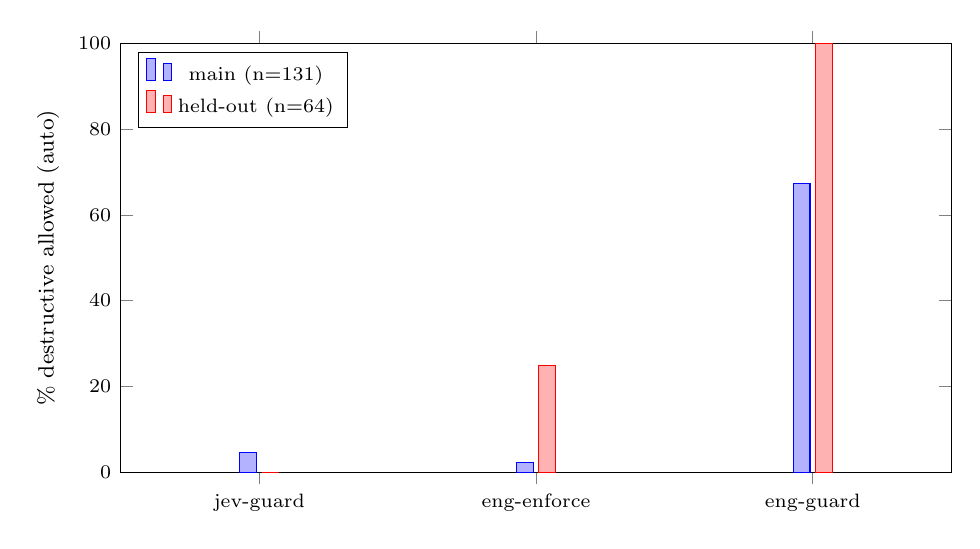
\begin{tikzpicture}
\begin{axis}[width=\columnwidth,height=0.58\columnwidth,ybar,bar width=6pt,
  symbolic x coords={jev-guard,eng-enforce,eng-guard},xtick=data,
  ymin=0,ymax=100,ylabel={\% destructive allowed (auto)},
  x tick label style={font=\scriptsize},label style={font=\footnotesize},
  tick label style={font=\scriptsize},
  legend style={font=\scriptsize,at={(0.02,0.98)},anchor=north west},
  enlarge x limits=0.25]
\addplot coordinates {(jev-guard,4.6)(eng-enforce,2.3)(eng-guard,67.2)};
\addlegendentry{main (n=131)}
\addplot coordinates {(jev-guard,0)(eng-enforce,25)(eng-guard,100)};
\addlegendentry{held-out (n=64)}
\end{axis}
\end{tikzpicture}
\caption{Under host auto-approval, the fraction of clearly-destructive calls each real gate
executes. Under the default (confirming) host mode all three are at 0\%. The gate-mode
$\times$ host-mode combination, not the model, governs protection.}
\label{fig:live}
\end{figure}

\textbf{Findings.} Table~\ref{tab:live} and Fig.~\ref{fig:live} give the paper's sharpest
result. Under the default
mode every gate leaks \emph{zero} destructive calls, because ``defer''/``ask'' surfaces a
prompt: the safety is the host's, not the gate's. Switch to auto-approval and the same gate
in \code{guard} mode auto-allows \textbf{88 of 131} clearly-destructive calls on the main
corpus and \textbf{64 of 64} on held-out adversarial families, because its ``ask'' verdicts
are silently downgraded to ``allow''; the identical gate in \code{enforce} mode leaks 3 and
16. One flag, a 29$\times$ difference in destructive calls executed. A probabilistic gate's
protection is a property of the gate-mode $\times$ host-mode combination, not of the model's
judgment, which mostly resolves to ``ask'' and is only as safe as whatever the ``ask'' is
wired to.

\begin{table}[t]
\caption{Destructive calls allowed, live, by host permission mode.}
\label{tab:live}
\centering\small\setlength{\tabcolsep}{4.5pt}
\begin{tabular}{@{}lcccc@{}}
\toprule
 & \multicolumn{2}{c}{main (n=131)} & \multicolumn{2}{c}{held-out (n=64)} \\
Gate (config) & default & auto & default & auto \\
\midrule
jev-guard & 0 & 6 & 0 & 0 \\
jev-engineering (enforce) & 0 & 3 & 0 & 16 \\
jev-engineering (guard) & 0 & \textbf{88} & 0 & \textbf{64} \\
\bottomrule
\end{tabular}
\end{table}

\section{A Certified-Threshold Recipe (the fix)}
\label{sec:fix}
The corpus criticism (thresholds copied without derivation) demands a constructive answer.
We give one that needs no training and ${\sim}40$ labelled calls. For a candidate allow
threshold $t$, the auto-allowed set is $\{p_{\text{safe}}\geq t\}$; a one-sided
Clopper--Pearson upper bound~\cite{clopper1934} on the fraction of that set that is actually
unsafe turns the observed count into a distribution-free $1{-}\delta$ bound on the true
false-allow rate. Choose the lowest $t$ whose bound is within a stated budget $\alpha$: the
most automation that still certifies the budget. The bound holds for any score; calibration
only affects how much coverage a given $\alpha$ buys.

\begin{figure}[t]
\centering
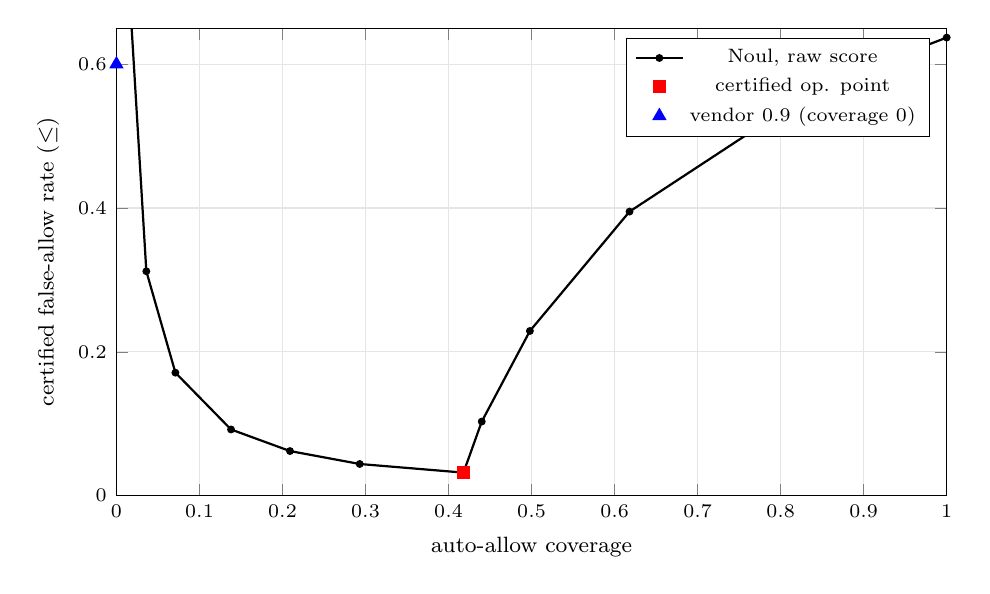
\begin{tikzpicture}
\begin{axis}[width=\columnwidth,height=0.62\columnwidth,
  xlabel={auto-allow coverage},ylabel={certified false-allow rate ($\leq$)},
  xmin=0,xmax=1,ymin=0,ymax=0.65,grid=both,grid style={gray!20},
  legend style={font=\scriptsize,at={(0.98,0.98)},anchor=north east},
  label style={font=\footnotesize},tick label style={font=\scriptsize}]
\addplot[thick,mark=*,mark size=1pt] coordinates {
 (0,1.0)(0.036,0.312)(0.071,0.171)(0.138,0.092)(0.209,0.062)(0.293,0.044)
 (0.418,0.032)(0.44,0.103)(0.498,0.229)(0.618,0.395)(0.849,0.570)(1.0,0.637)};
\addlegendentry{Noul, raw score}
\addplot[only marks,mark=square*,mark size=2.2pt,red] coordinates {(0.418,0.032)};
\addlegendentry{certified op. point}
\addplot[only marks,mark=triangle*,mark size=2.6pt,blue] coordinates {(0.0,0.60)};
\addlegendentry{vendor $0.9$ (coverage 0)}
\end{axis}
\end{tikzpicture}
\caption{Certified false-allow rate versus auto-allow coverage as the threshold sweeps
(distribution-free Clopper--Pearson upper bound, $\delta{=}0.05$, 225 definite items,
\code{jev-1.13.0}). The
vendor's $0.9$ sits at zero coverage; a data-chosen threshold certifies 42\% coverage at
$\leq 3.1\%$ false-allow.}
\label{fig:curve}
\end{figure}

On our data the vendor's fixed $0.9$ certifies \emph{zero} coverage (it allows nothing;
Fig.~\ref{fig:curve}). A
data-chosen threshold on the same 225 definite items certifies \textbf{42\% auto-allow at a
$\leq 3.1\%$ false-allow rate} ($\delta=0.05$), auto-allowing all 94 clearly-safe items.
The vendor's own $0.9$ works once scores are isotonically recalibrated (41\% coverage,
$\leq 3.2\%$), so $0.9$ was not a wrong number but a number on the wrong scale: fix the scale
or fix the number, but copying the number and doing neither yields a dead gate. On
\code{jev-1.14.0} the recipe certifies the same 42\% at $\leq 3.1\%$, but at a different
threshold ($0.285$, not $0.245$), while $0.9$ now auto-allows 11\% yet certifies only
$\leq 11.3\%$: a certified threshold is tied to a model version and must be re-derived when
it changes. Honestly, a
$2\%$ budget certifies nothing here---94 clean calibration points bound the rate only to
${\sim}3\%$---which is itself the useful guidance: tighter budgets need more calibration
data.

\textbf{Label reliability.} An independent re-adjudication of a stratified 88-item sample,
blind to the generation rule, agrees with the corpus on the safe-vs-unsafe distinction at
$\kappa=0.86$ with \emph{zero} severity inversions; all disagreement lies on the
``ask-vs-auto-handle'' boundary, a documented policy choice, giving a moderate three-way
$\kappa=0.47$.

\section{Generalization Beyond Jev}
\label{sec:general}
Two facts argue the findings are not vendor-specific. First, the host itself fails open: the
coding-agent hook mechanism these gates run on does not block a timed-out
hook~\cite{cchooks}, so a stalled model judge is overridden into fail-open regardless of
vendor. The host now offers an opt-in \code{onFailure} setting that blocks instead; the default is unchanged. Second, a small non-Jev comparison set reproduces every pathology: a REST-judge gate
exposes fail-open as an environment toggle (mirroring the mode flag above), fails closed on
its command path but open on its URL path (mirroring split behaviour we observed), and once
``quietly downgraded require-approval to allow'' (mirroring the live 88/131 downgrade). By
contrast, deterministic gates in the same set have no availability axis at all---nothing to
switch off with a padded input. The pathologies are properties of putting a probabilistic
model in the authorization path, which Jev popularized but does not own.

\section{Five Weeks Later}
\label{sec:recheck}
We re-checked every finding on 2026-10-31, five weeks after measurement, by reading each
gate's upstream code and re-running the benchmark on the current model. \textbf{Gates.}
Four of the five gates in Sec.~\ref{sec:fault} changed. jev-belay and jev-guard still
proceed or defer on every model failure, and jev-guard's action path still sends the full,
untruncated input, so the padding bypass still applies. jev-engineering added deterministic
deny rules that now catch our padded credential-exfiltration probe before any model
call---a deterministic layer closing what the probabilistic one left open---but its
fallback on model failure is unchanged, and it gained an \code{auto} mode in which the
model's verdict alone skips the human prompt. jev-harness moved the other way: its TypeSafe
path, fail-closed when measured, now by default decides on an offline engine when the model
fails, marking the answer as degraded but acting on it. \textbf{Ecosystem.} The index we
sampled grew from 49 to 66 candidates. Of the readable new action gates, the hook-style one
documents fail-open on every failure and all ship undocumented threshold constants, while two
non-hook gates fail closed. \textbf{Host.} A timed-out hook still does not block by default;
an opt-in to block now exists. The mechanisms persist; what moved is the model scale
(Sec.~\ref{sec:bench}) and, in one gate, the failure default toward open.

\section{Threats to Validity}
The corpus is a convenience sample from one curated index, collected in the first two weeks
of a single-vendor ecosystem; prevalence numbers should be read as launch-window evidence, and the non-Jev
comparison establishes mechanism transfer, not off-Jev prevalence. Benchmark labels derive
from generation rules; we mitigate with disputable-item flags, sensitivity analyses, and the
independent re-adjudication above. The benchmark measures our gate configurations, not each
deployed gate's exact wording; Sec.~\ref{sec:live} closes this for three gates by running
their real code. The benchmark covers two model versions; fault injection and the live cross-evaluation used
\code{jev-1.13.0} at pinned gate commits, and their re-check at upstream HEAD is by code
reading (Sec.~\ref{sec:recheck}). We study per-call gates only; violations that span several individually allowed calls are
beyond any per-action monitor~\cite{localallow2026}. Fault
classifications are now observed, not merely read.

\section{Conclusion}
Practitioners are building agent authorization out of a remote, probabilistic model, against
the security literature's advice, and the result fails in ways an operator cannot see from
the outside. The model can separate safe from dangerous perfectly and the gate can still be
useless: a copied threshold that never fires, or fires differently after a silent model update, an ``ask'' silently downgraded to ``allow,'' a
padded command that switches the gate off. The safety that remains is usually the host's
confirmation prompt, not the model. Where a probabilistic model is used, its threshold should
be certified from data with an explicit false-allow budget against a pinned model version,
and re-certified when that version changes; its failure path should be closed, not open. We release the corpus, benchmark, fault harness, live-evaluation runner,
and threshold recipe to make these properties measurable for the next gate.


\bibliographystyle{IEEEtran}
\bibliography{refs}
\end{document}
